\documentclass{scrbook}

\usepackage[utf8]{inputenc}
\usepackage[T1]{fontenc}

% ##################################################
% Dokumentvariablen
% ##################################################

% Persoenliche Daten
\newcommand{\docNachname}{Nachname}
\newcommand{\docVorname}{Vorname}
\newcommand{\docStrasse}{Straße}
\newcommand{\docOrt}{Ort}
\newcommand{\docPlz}{PLZ}
\newcommand{\docEmail}{Mail}
\newcommand{\docMatrikelnummer}{Matrikel}

% Dokumentdaten
\newcommand{\docTitel}{Titel}
\newcommand{\docUntertitel}{Untertitel}
\newcommand{\docArtDerArbeit}{Art der Arbeit}
\newcommand{\docStudiengang}{Studiengang}
\newcommand{\docAbgabedatum}{Abgabedatum}
\newcommand{\docErsterReferent}{Erster Referent}
\newcommand{\docZweiterReferent}{Zweiter Referent}

% ##################################################
% Allgemeine Pakete
% ##################################################

% Abbildungen einbinden
\usepackage{graphicx}
\usepackage{minipage-marginpar}

% Paket zur Index-Erstellung (Schlagwortverzeichnis)
\usepackage{imakeidx}
\makeindex[intoc, title=Schlagwortverzeichnis, columns=1]
\indexsetup{
	headers={\indexname}{\indexname}
}

% Farben
\usepackage{color}
\usepackage[usenames,dvipsnames,svgnames,table]{xcolor}

% Maskierung von URLs und Dateipfaden
\usepackage[hyphens]{url}

% Deutsche Unterstützung
\usepackage[ngerman]{babel}

% Mathematische Zeichen etc.
\usepackage{amsmath}
\usepackage{amssymb}

% ##################################################
% Seitenformatierung
% ##################################################

\KOMAoption{paper}{A4}
\KOMAoption{twoside}{true}

\usepackage[
	portrait,
	top = 3cm,
	bottom = 2cm,
	inner = 2.5cm,
	outer = 2.5cm,
	bindingoffset = 1.5cm,
]{geometry}


% ##################################################
% Kopf- und Fusszeile
% ##################################################

\usepackage[singlespacing = true]{scrlayer-scrpage}
\clearpairofpagestyles

\KOMAoption{headsepline}{true}
\KOMAoption{plainheadsepline}{true}

\ohead*{\pagemark} % Seitennummer außen
\ihead*{\leftmark} % Kapitel innen

\setkomafont{pageheadfoot}{\bfseries} % Kopfzeile fett
\setkomafont{pagination}{\bfseries} % Seitenzahl fett


% ##################################################
% Absätze
% ##################################################

\KOMAoption{parskip}{half}

% Absätze der Überschriften anpassen
\RedeclareSectionCommand[afterskip = \baselineskip]{chapter}
\RedeclareSectionCommand[beforeskip = \baselineskip, afterskip = 1sp]{section}
\RedeclareSectionCommand[beforeskip = \baselineskip, afterskip = 1sp]{subsection}

% ##################################################
% Schriften
% ##################################################

% Erlaubt beliebig große Schrift
\usepackage{lmodern}

% Schriftgröße
\KOMAoption{fontsize}{12pt}

% Stdandardschrift festlegen
\renewcommand*{\familydefault}{\sfdefault}

% Standard Zeilenabstand: 1,5 zeilig
\usepackage{setspace}
\onehalfspacing 

% Schriftgroessen festlegen
\setkomafont{chapter}{\large\bfseries} 
\setkomafont{section}{\normalsize\bfseries} 
\setkomafont{subsection}{\normalsize\mdseries} 
\setkomafont{caption}{\normalsize\mdseries} 

% ##################################################
% Inhaltsverzeichnis / Allgemeine Verzeichniseinstellungen
% ##################################################

\KOMAoption{toc}{chapterentrywithdots}
\KOMAoption{listof}{nochaptergap, entryprefix}

% Einträge für andere Verzeichnisse
\setuptoc{toc}{totoc}
\KOMAoption{toc}{listof, index, bibliography}

% Schriftart und -groesse im Inhaltsverzeichnis anpassen
\setkomafont{chapterentry}{\normalsize}

% Zeilenabstand in den Verzeichnissen einstellen
\BeforeStartingTOC[toc]{
	\DeclareTOCStyleEntry[
		beforeskip=.5\baselineskip
	]{tocline}{chapter}
	
	\DeclareTOCStyleEntry[
		beforeskip=.5\baselineskip
	]{tocline}{section}
	
	\renewcommand*{\autodot}{}
}


% ##################################################
% Allgemeine Abbildungs- und Tabellenverzeichnis Optionen
% ##################################################

% Pakete für Tabellen und Abbildungen
\usepackage{chngcntr}
\usepackage{caption}
\usepackage{subcaption}

% ##################################################
% Abbildungsverzeichnis und Abbildungen
% ##################################################

\usepackage{wrapfig}

% Nummerierung von Abbildungen
\counterwithout{figure}{chapter}

\BeforeStartingTOC[lof]{
	\DeclareTOCStyleEntry[
		beforeskip=.5\baselineskip,
		numwidth=10em
	]{tocline}{figure}
	
	\renewcommand*{\autodot}{:}
}


% ##################################################
% Tabellenverzeichnis und Tabellen
% ##################################################

\usepackage{booktabs}

% Nummerierung von Tabellen
\counterwithout{table}{chapter}

\BeforeStartingTOC[lot]{
	\DeclareTOCStyleEntry[
		beforeskip=.5\baselineskip,
		numwidth=10em
	]{tocline}{table}
	
	\renewcommand*{\autodot}{:}
}


% ##################################################
% Listings (Quellcode)
% ##################################################

\usepackage{minted}
\usepackage[babel, german=quotes]{csquotes}
\MakeOuterQuote{"}

\renewcommand{\listoflistingscaption}{Quellcodeverzeichnis}
\renewcommand{\listingscaption}{Quellcode}
\newcommand{\listingautorefname}{Quellcode}

\renewcommand*{\listoflistings}{\listoftoc[{\listoflistingscaption}]{lol}}
\setuptoc{lol}{totoc}

\BeforeStartingTOC[lol]{
	\DeclareTOCStyleEntry[
		level=1,
		indent=1.5em,
		numwidth=10em,
		beforeskip=.5\baselineskip,
		entrynumberformat=\listingscaption~,
	]{tocline}{listing}
	
	\renewcommand*{\autodot}{:}
}

% ##################################################
% Theoreme
% ##################################################

% Umgebung für Formeln
\newtheorem{formel}{Formel}
\newcommand{\formelautorefname}{Formel}
  	
% ##################################################
% Literaturverzeichnis
% ##################################################

\usepackage[
	backend = biber,
	bibstyle = authoryear,
	citestyle = authoryear,
	giveninits = true,
	uniquename = false,
	dashed = false,
]{biblatex}

\DeclareNameAlias{sortname}{family-given}

\DefineBibliographyStrings{ngerman}{
	bibliography = {{Literaturverzeichnis}},
	andothers = {{et al.}},
	mathesis = {{Masterarbeit}},
}

\addbibresource{meta/literature.bib}

% ##################################################
% PDF / Dokumenteninterne Links
% ##################################################

\usepackage[
	colorlinks=false,
   	linkcolor=black,
   	citecolor=black,
  	filecolor=black,
	urlcolor=black,
    bookmarks=true,
    bookmarksopen=true,
    bookmarksopenlevel=3,
    bookmarksnumbered,
    plainpages=false,
    pdfpagelabels=true,
    hyperfootnotes,
    pdftitle ={\docTitel},
    pdfauthor={\docVorname \docNachname},
    pdfcreator={\docVorname \docNachname}
]{hyperref}

% ##################################################
% Abkürzungen
% ##################################################

\usepackage[acronym, nogroupskip, nonumberlist, nopostdot, translate=babel]{glossaries}
\makenoidxglossaries
\loadglsentries{meta/glossary}

% Fettgedruckte Abkürzung im Verzeichnis
\renewcommand*{\glsnamefont}[1]{\textbf{#1}}


% ##################################################
% Anhang
% ##################################################

\newcommand*{\appendixstyle}{
	\renewcommand*{\raggedchapter}{\centering}
	\RedeclareSectionCommand[font=\Huge, beforeskip=0.4\textheight]{chapter}
	
	\RedeclareSectionCommand[font=\large, beforeskip=0pt, afterskip=1sp]{section}
	
	\RedeclareSectionCommand[font=\bfseries, beforeskip=0pt, afterskip=1sp]{subsection}
}



\begin{document}

\setcounter{secnumdepth}{3}

% ##################################################
% Startteil
% ##################################################

% Titelblatt
\begin{titlepage}
\pagestyle{empty}

% ##################################################
% HFU- und Firmen-Logo einbinden
% ##################################################
\begin{minipage}{0.45\textwidth}
	\flushleft
	% Firmenlogo
	% \includegraphics{path/to/firmenlogo}
\end{minipage}
\hfill
\begin{minipage}{0.45\textwidth}
	\flushright
	
\includegraphics[height=2.5cm]{content/logos/hfu.jpg}
\end{minipage}
\vspace*{2em}

% ##################################################
% Titel
% ##################################################
\begin{center}
{\fontsize{18}{22}\selectfont \docArtDerArbeit}\\[5mm]
{\fontsize{18}{22}\selectfont im Studiengang} \\[5mm]
{\fontsize{18}{22}\selectfont \docStudiengang}\\
\vspace*{4em}
\begin{onehalfspace}
{\fontsize{22}{26}\selectfont \textbf{\docTitel}}\\[5mm]
{\fontsize{18}{22}\selectfont \docUntertitel}
\end{onehalfspace}
\end{center}

% ##################################################
% Zusatzinformationen
% ##################################################
\vfill
\begin{center}
\begin{tabular}{lcl}
Referent  		&:& \docErsterReferent 	\\ \\
Koreferent 		&:& \docZweiterReferent \\ \\
Vorgelegt am 	&:& \docAbgabedatum 	\\ \\
Vorgelegt von 	&:& \docVorname{} \docNachname\\
				& & Matrikelnummer: \docMatrikelnummer\\
				& & \docStrasse, \docPlz{} \docOrt\\
				& & \docEmail		
\end{tabular}
\end{center}
\end{titlepage}

\cleardoubleemptypage

\frontmatter
\pagenumbering{Roman}

% Abstract
\chapter*{Abstract\markboth{Abstract}{Abstract}}
\addcontentsline{toc}{chapter}{Abstract}

[Abstract Englisch]

[Abstract Deutsch]

\cleardoubleemptypage

% Inhaltsverzeichnis
\tableofcontents
\cleardoubleemptypage

% Abbildungsverzeichnis einbinden
\listoffigures
\cleardoubleemptypage

% Tabellenverzeichnis einbinden
\listoftables
\cleardoubleemptypage

% Quellcodeverzeichnis einbinden
\listoflistings
\cleardoubleemptypage

% Abkürzungsverzeichnis
\setglossarystyle{long}

\renewcommand*{\arraystretch}{1.5} % 1.5-facher Zeilenabstand
\printnoidxglossary[type=\acronymtype, title={Abkürzungsverzeichnis}]
\renewcommand*{\arraystretch}{1.0} % Einfacher Zeilenabstand

% ##################################################
% Hauptteil
% ##################################################
\mainmatter

% Abbildungs- und Tabellennummerierung zurücksetzen
\setcounter{figure}{0}
\setcounter{table}{0}

% Kapitel
\chapter{Einleitung}
Dies ist ein Minimalbeispiel für eine wissenschaftliche Arbeit an der Fakultät Informatik der \acrshort{hfu}.

\section{Abkürzungen}
\index{Abkürzung}
Abkürzungen werden in der Datei "glossary.tex" mit dem Befehl \mintinline{latex}{\newacronym} deklariert.
Im Text werden diese mit dem Befehl \mintinline{latex}{\gls} verwendet.

Beispielsweise kann die Abkürzung der Hochschule deklariert werden mit
\mint{latex}{\newacronym{hfu}{HFU}{Hochschule Furtwangen}}

Bei Erstverwendung es \mintinline{latex}{\gls} Befehls wird die volle Abkürzung ausgeschrieben, wie folgt:
\gls{hfu}.
Bei späterer Verwendung wird nur die Kurzform gedruckt: \gls{hfu}.

Soll eine spezifische Form der Abkürzung verwendet werden, gibt es noch die Befehle \mintinline{latex}{\acrfull}, \mintinline{latex}{\acrshort} und \mintinline{latex}{\acrlong}.

\section{Tabellen}
\index{Tabelle}
Tabellen werden in ein \mintinline{latex}{table}-Environment eingebettet.
Die Tabelle und Überschrift werden mit \mintinline{latex}{\centering} auf der Seite horizontal zentriert.
Die Überschrift wird mit \mintinline{latex}{\caption} über der Tabelle platziert.

Die Tabelle selbst wird mit einem \mintinline{latex}{tabular}-Environment angelegt.
Die verfügbaren Optionen für die Spaltenformattierungen des \mintinline{latex}{tabular}-Environments sind in \autoref{tab:table_options} aufgelistet.

\begin{table}
	\centering
	\caption{Verfügbare Optionen für die Spalten bei einer Tabelle}
	\label{tab:table_options}
	\begin{tabular}{ll}
		\toprule
		Option & Funktion \\
		\midrule
		l & linksbündig \\
		c & zentriert \\
		p\{breite\} & linksbündig mit fester Breite \\
		\bottomrule
	\end{tabular}
\end{table}

Horizontale Trennlinien lassen sich mit \mintinline{latex}{\toprule}, \mintinline{latex}{\midrule} und \mintinline{latex}{\bottomrule} setzen, entsprechend der Position.
Von vertikalen Trennlinien sollte abgesehen werden.

Die Zellen der Tabelle werden zeilenweise geschrieben.
Die Spalten werden mit \mintinline{latex}{&} getrennt, eine Zeile wird mit \mintinline{latex}{\\} abgeschlossen.

\section{Abbildungen}
\index{Abbildung}
Ähnlich wie Tabellen werden Abbildungen in das \mintinline{latex}{figure}-Environment eingebettet.
Ebenfalls wird die Abbildung mit Unterschrift durch den Befehl \mintinline{latex}{\centering} zentriert.

Die Abbildung selbst wird eingebunden mit 
\mint{latex}{\includegraphics[width=0.7\linewidth]{path/to/image}}
Die Unterschrift wird mit \mintinline{latex}{\caption} unter dem Bild platziert.

\begin{figure}
	\centering
	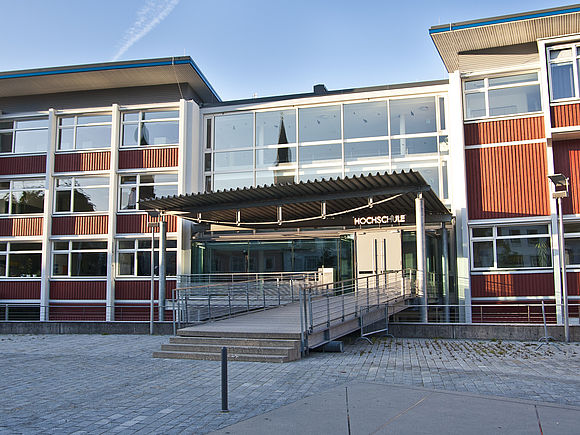
\includegraphics[width=0.7\linewidth]{content/pictures/hfu_a_bau}
	\caption{A-Bau der HFU, Campus Furtwangen}
	\label{fig:hfu_a_bau}
\end{figure}

\begin{wrapfigure}{r}{0.4\linewidth}
	\centering
	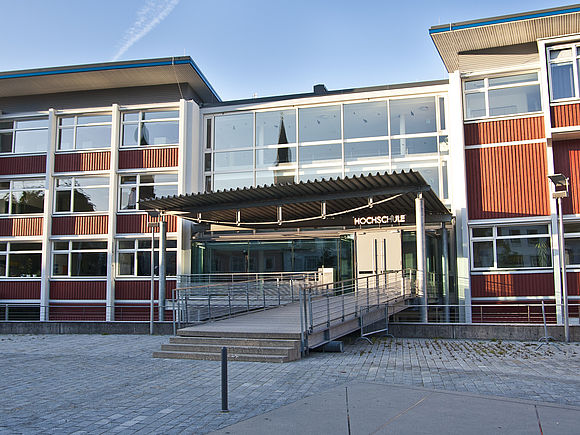
\includegraphics[width=0.8\linewidth]{content/pictures/hfu_a_bau}
	\caption{A-Bau der HFU, Campus Furtwangen}
	\label{fig:hfu_a_bau_wrap}
\end{wrapfigure}

\index{Abbildung!neben Text}
Alternativ kann eine Abbildung auch mit dem \mintinline{latex}{wrapfigure}-Environment neben dem Text platziert werden.
Dazu wird zusätzlich die Ausrichtung (\mintinline{latex}{l}/\mintinline{latex}{r}) und die Breite angegeben.

\section{Quellcode}
\index{Quellcode}
Quellcode kann in verschiedenen Formen eingebunden werden:

\begin{itemize}
	\item Inline
	\item Einzeiler
	\item Mehrzeiler
\end{itemize}

\index{Quellcode!inline}
Für inline-code wird der Befehl \mintinline{latex}{\mintinline{language}{code}} verwendet.
\index{Quellcode!einzeilig}
Analog wird für Einzeiler der Befehl
\mint{latex}{\mint{language}{code}}
verwendet.

\index{Quellcode!mehrzeilig}
Mehrzeiliger Quellcode wird in ein \mintinline{latex}{listing}-Environment eingebettet.
Die \mintinline{latex}{\caption} wird dabei unter dem Quellcode platziert.
Der Quellcode selbst wird inerhalb eines \mintinline{latex}{minted}-Environment geschrieben.
In \autoref{lis:multiline_code} ist beispielsweise der Code programmiert, der diese Ausgabe produziert.

\begin{listing}
\begin{minted}[linenos, tabsize=4]{latex}
\begin{listing}
	\begin{minted}[linenos, tabsize=4]{latex}
		...
	\end {minted}
	\caption{Multiline Quellcode}
	\label{lis:multiline_code}
\end{listing}
\end{minted}
\caption{Multiline Quellcode}
\label{lis:multiline_code}
\end{listing}

Zum Anzeigen von Zeilennummern wird die Option \mintinline{latex}{linenos} verwendet, zum Einstellen der Tab-Breite wird \mintinline{latex}{tabsize} spezifiziert.

\section{Referenzen}
\label{sec:references}
Textteile, Abbildungen, Tabellen und Quellcode kann im Text referenziert werden.
Dazu muss bei entsprechender Textstelle, Abbildung, Tabelle oder Quellcode mit \mintinline{latex}{\label{key}} ein Label gesetzt werden.
Dieses Label wird mit \mintinline{latex}{\ref{key}} referenziert.
Dabei wird die Aktuelle Kapitelnummer, Abbildungsnummer etc. angezeigt.

Für eine volle Referenz kann \mintinline{latex}{\autoref{key}} verwendet werden.
Bei einer Referenz auf den Aktuellen Abschnitt wird beispielsweise die Ausgabe "\autoref{sec:references}" erzeugt.

\section{Zitate}
Da dieses Thema umfangreicher ist sollte die Dokumentation von BibLaTeX herangezogen werden \parencite{biblatex}.



% ##################################################
% Schlussteil
% ##################################################

% Schlagwortverzeichnis
\printindex

% Literaturverzeichnis
\singlespacing
\printbibliography[
	heading = bibintoc,
]

% Eidesstattliche Erklärung
\chapter*{Eidesstattliche Erklärung\markboth{Eidesstattliche Erklärung}{Eidesstattliche Erklärung}}
\addcontentsline{toc}{chapter}{Eidesstattliche Erklärung}

Ich versichere, dass ich die vorstehende Arbeit selbständig verfasst und hierzu keine anderen als die angegebenen Hilfsmittel verwendet habe.
Alle Stellen der Arbeit die wörtlich oder sinngemäß aus fremden Quellen entnommen wurden, sind als solche kenntlich gemacht.

Die Arbeit wurde bisher in gleicher oder ähnlicher Form in keinem anderen Studiengang als Prüfungsleistung vorgelegt oder an anderer Stelle veröffentlicht.

Ich bin mir bewusst, dass eine falsche Erklärung rechtliche Folgen haben kann.

\vspace*{1.5cm}
\line(1,0){275}

\docOrt, den  \docAbgabedatum ~~\docVorname~\docNachname



% Anhang
\appendix
\appendixstyle

% Hier Anhang einfügen
\chapter{Monatsberichte}
\cleardoubleemptypage

\section*{Januar (01.01.2020 - 31.01.2020)}
\subsection*{Durchgeführte Arbeiten}
\begin{addmargin}{1cm}
	[13--15 Zeilen]
\end{addmargin}


\subsection*{Erzielte Ergebnisse}
\begin{addmargin}{1cm}
	[8--10 Zeilen]
\end{addmargin}


\subsection*{Abweichungen}
\begin{addmargin}{1cm}
	[6--8 Zeilen]
\end{addmargin}

\subsection*{Ausblick}
\begin{addmargin}{1cm}
	[4--6 Zeilen]
\end{addmargin}
\clearpage




\end{document}
